\documentclass[10pt]{beamer}

\usepackage[T1]{fontenc}
\usepackage{lmodern}
\usepackage[british]{babel}
\usepackage{microtype}
\usepackage{mathtools,amsmath,amssymb}

\usepackage{tikz}
\usepackage{pgfplots}
\usepackage{graphicx}
\usepackage[dvipsnames]{xcolor}
\usepackage{qrcode}
\usepackage{dsfont}
\usepackage{appendixnumberbeamer}

\usepackage{hyperref}
\usepackage{caption,subcaption}
\captionsetup{
    font=scriptsize,
    labelfont=scriptsize,
    margin=2em
}

\usepackage{csquotes}
\usepackage[backend=biber, style=authoryear]{biblatex}
\addbibresource{refs.bib}
\AtEveryCitekey{% footnote citations: authors (I D Couzin style), year, title and journal
    \DeclareNameAlias{sortname}{given-family}%
    \DeclareNameAlias{default}{given-family}%
    \toggletrue{abx@bool@giveninits}%
    \renewrobustcmd*{\bibinitperiod}{}%
    \renewrobustcmd*{\bibinithyphendelim}{\mbox{-}}%
    \clearfield{booktitle}%
    \clearfield{volume}%
    \clearfield{number}%
    \clearfield{pages}%
    \clearfield{note}%
    \clearfield{eprint}%
    \clearlist{publisher}%
    \clearlist{location}%
    \clearlist{organization}%
    \renewbibmacro{in:}{}%
}

\usepackage[default]{sourcesanspro}
\usetheme[progressbar=none, sectionpage=none]{moloch}

\definecolor{beamercolor}{HTML}{4F7892}
\definecolor{altcolor}{HTML}{B84A62}

\setbeamercolor{frametitle}{bg=white, fg=beamercolor!75!black}
\setbeamercolor{title separator}{fg=altcolor}
\setbeamercolor{structure}{fg=beamercolor}
\setbeamertemplate{page number in head/foot}[totalframenumber]
\setbeamertemplate{caption}[default]
\makeatletter   % blocks with an empty title get a thin line instead of the title band
\newcommand{\untitledblockbegin}[2]{%
    \par\vskip\medskipamount%
    \ifx\insertblocktitle\@empty
        {\usebeamercolor[bg]{#1}\moveleft.75ex\vbox{\hrule width \dimexpr\linewidth+1.5ex\relax height 3pt}}\nointerlineskip
    \else
        \begin{beamercolorbox}[colsep*=.75ex]{#1}%
            \usebeamerfont*{block title}\insertblocktitle%
        \end{beamercolorbox}\noframebreak%
        {\parskip0pt\par}\nointerlineskip\vskip-0.5pt%
    \fi
    \usebeamerfont{block body}%
    \begin{beamercolorbox}[colsep*=.75ex,vmode]{#2}%
        \vskip-.75ex\vbox{}}
\makeatother
\setbeamertemplate{block begin}{\untitledblockbegin{block title}{block body}}
\setbeamertemplate{block alerted begin}{\untitledblockbegin{block title alerted}{block body alerted}}
\setbeamertemplate{block example begin}{\untitledblockbegin{block title example}{block body example}}

\setbeamercolor{block title}{bg=beamercolor!18, fg=beamercolor!70!black}
\setbeamercolor{block body}{bg=beamercolor!6, fg=black}
\setbeamercolor{block title alerted}{bg=altcolor!18, fg=altcolor!75!black}
\setbeamercolor{block body alerted}{bg=altcolor!6, fg=black}
\setbeamercolor{alerted text}{fg=altcolor}
\setbeamerfont{footnote}{size=\tiny}
\setbeamerfont{date}{size=\scriptsize}
\setbeamerfont{institute}{size=\footnotesize}
\setbeamercolor{footnote mark}{fg=Blue}
\setbeamertemplate{footnote}{\parindent 1em\noindent\raggedright\hbox to 1.5em{\hfil\insertfootnotemark}\tiny\insertfootnotetext\par}
\renewcommand{\footnoterule}{}
\setbeamertemplate{frametitle continuation}{}
\setbeamerfont{bibliography item}{size=\tiny, shape=\upshape, series=\mdseries}
\setbeamerfont{bibliography entry author}{size=\tiny, shape=\upshape, series=\mdseries}
\setbeamerfont{bibliography entry title}{size=\tiny, shape=\upshape, series=\mdseries}
\setbeamerfont{bibliography entry location}{size=\tiny, shape=\upshape, series=\mdseries}
\setbeamerfont{bibliography entry note}{size=\tiny, shape=\upshape, series=\mdseries}

\newcommand{\vect}[1]{\mathbf{#1}}

\newcommand {\bx} {{\vect{x}}}
\newcommand {\by} {{\vect{y}}}
\newcommand {\bz} {{\vect{z}}}
\newcommand {\bv} {{\vect{v}}}
\newcommand {\bw} {{\vect{w}}}
\newcommand {\bu} {{\vect{u}}}
\newcommand {\be} {{\vect{e}}}

\newcommand {\BX} {{\vect{X}}}
\newcommand {\BY} {{\vect{Y}}}
\newcommand {\BV} {{\vect{V}}}
\newcommand {\BU} {{\vect{U}}}
\newcommand {\BZ} {{\vect{Z}}}

\newcommand{\Bluecite}[1]{\textcolor{Blue}{#1}}
\newcommand{\ghostfootnote}[1]{{% footnote without a mark, for references that apply to the whole slide
    \renewcommand{\thefootnote}{}\footnote[frame]{#1}\addtocounter{footnote}{-1}}}

\newtheorem{proposition}{Proposition}
\newcommand {\Z}{\mathbb{Z}}
\newcommand {\R}{\mathbb{R}}
\newcommand {\T}{\mathbb{T}}
\newcommand*\diff{\mathop{}\!\mathrm{d}}
\newcommand*\dt{\diff t}
\newcommand*\dx{\diff \bx}
\newcommand*\dv{\diff \bv}
\newcommand*\dy{\diff \by}
\newcommand*\dw{\diff w}
\newcommand{\red}{\color{red}}
\newcommand{\blue}{\color{blue}}
\newcommand{\gray}{\color{Plum}}
\newcommand{\Red}[1]{\textcolor{BrickRed}{#1}}
\newcommand{\Blue}[1]{\textcolor{Blue}{#1}}
\newcommand{\Green}[1]{\textcolor{ForestGreen}{#1}}

% cell states, in the colours of the simulation figures
\definecolor{Bcolor}{HTML}{3A9B3A}
\definecolor{Ccolor}{HTML}{E09A1A}
\newcommand{\B}{\textcolor{Bcolor}{\textbf{B}}}
\newcommand{\C}{\textcolor{Ccolor}{\textbf{C}}}

\graphicspath{{figures/}}


\title{3D modelling of confined gastruloid aggregates}
\subtitle{An agent-based model of T/Bra patterning under confinement}
\author[victor.villegas@upc.edu]{Víctor Villegas-Morral}
\titlegraphic{
\includegraphics[height=2.5em]{figures/upc-mat-logo.pdf}}
\date[November 2026]{Lab meeting\\ November 2026}
\institute[]{Joint work with D. Oriola and V. Weichselberger}

\begin{document}

\frame{\titlepage}



\section{The experiment}

\begin{frame}{Gastruloids under confinement}
    \ghostfootnote{Images: V. Weichselberger.}
    \begin{columns}[c]
    \column{0.52\textwidth}
        \centering
        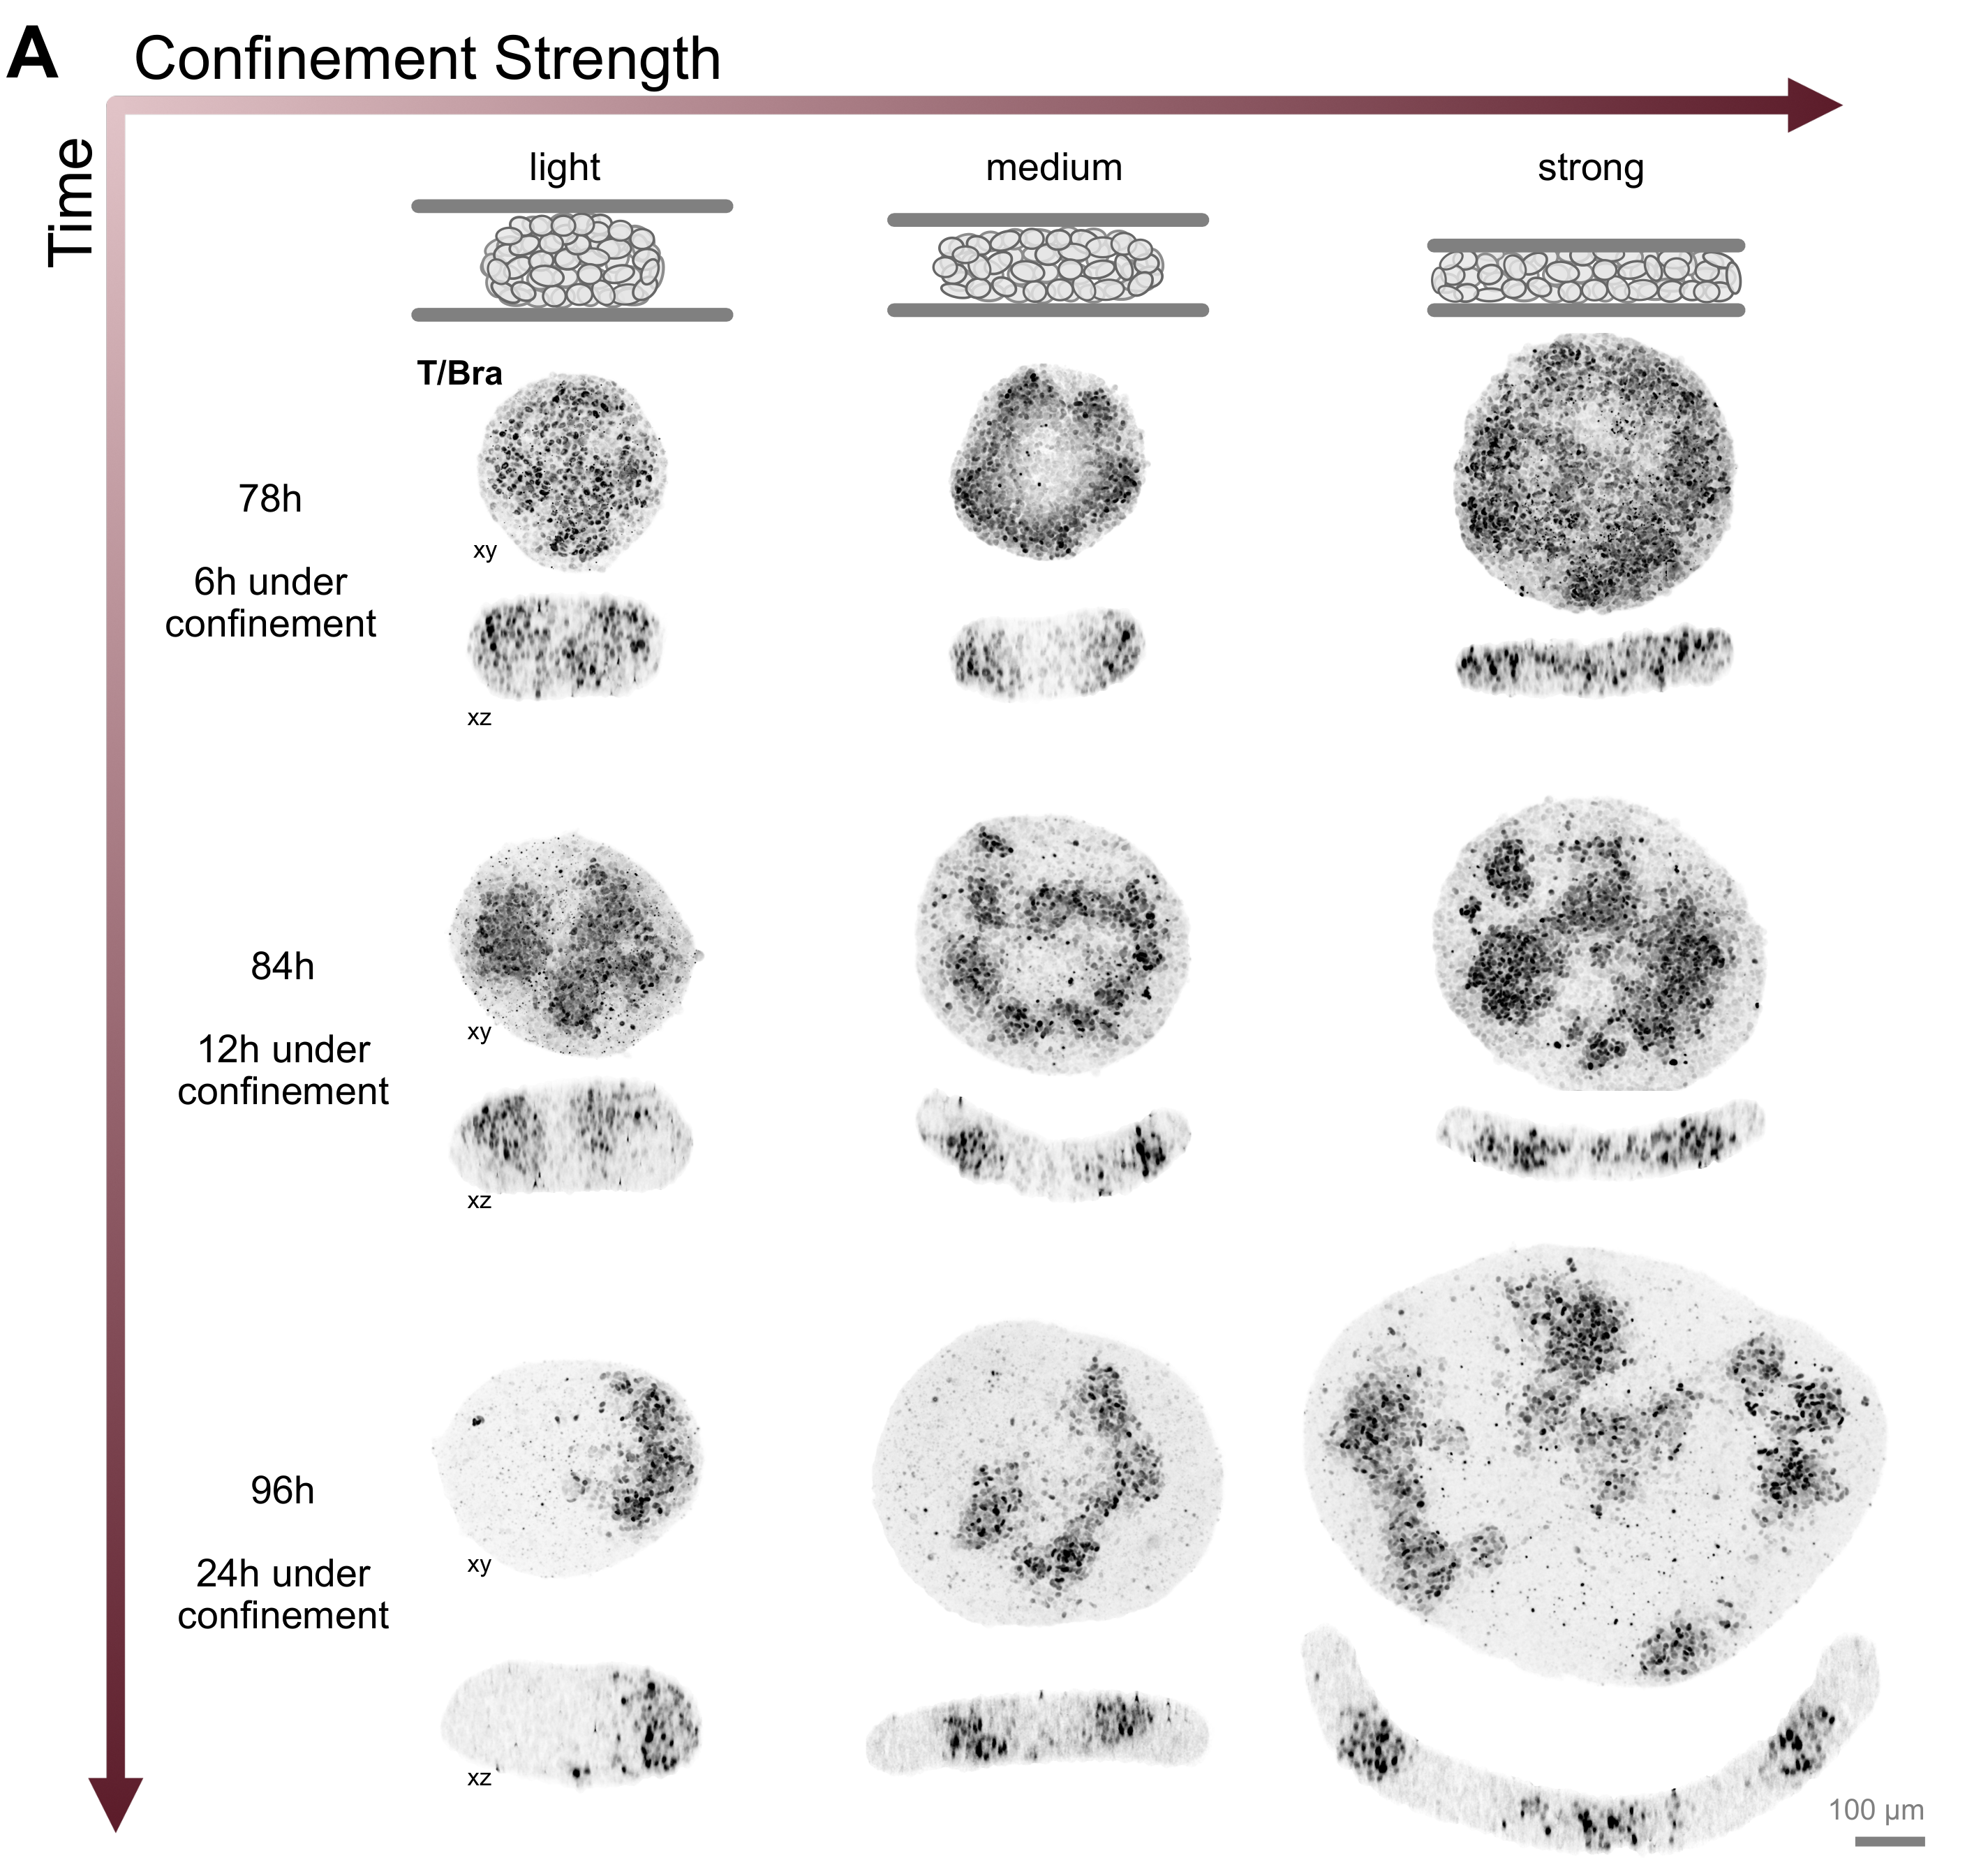
\includegraphics[width=\linewidth]{exp-confinement-time.png}
    \column{0.46\textwidth}
        \small
        Gastruloids are squeezed between two plates at 72\,h, right before T/Bra polarises, and read at 96\,h.
        \vspace{0.75em}
        \begin{itemize}
            \item<2-> \textbf{Light}: T/Bra polarises, as without confinement.
            \item<3-> \textbf{Medium}: T/Bra stays in the centre, sometimes as a ring.
            \item<4-> \textbf{Strong}: T/Bra breaks into clusters.
        \end{itemize}
        \vspace{0.75em}
        \only<5->{\begin{alertblock}{}
            The larger the gastruloid, the thicker the slab that still gives clusters.
        \end{alertblock}}
    \end{columns}
\end{frame}


\begin{frame}{Goal}
    \begin{block}{}
        A single model, with a single set of parameters, that reproduces
        \begin{itemize}
            \item polarisation without confinement,
            \item a central cluster under medium confinement,
            \item clusters under strong confinement,
            \item and the fusion of aggregates of the same and of different cell types.
        \end{itemize}
    \end{block}
    \pause
    \vspace{1em}
    \begin{alertblock}{}
        \centering
        \vspace{0.25em}
        What sets the outcome: the number of cells, the thickness of the slab, or both?
        \vspace{0.25em}
    \end{alertblock}
\end{frame}



\section{The model}

\begin{frame}{The model in one slide}
    \ghostfootnote{\fullcite{oriola}}
    \centering
    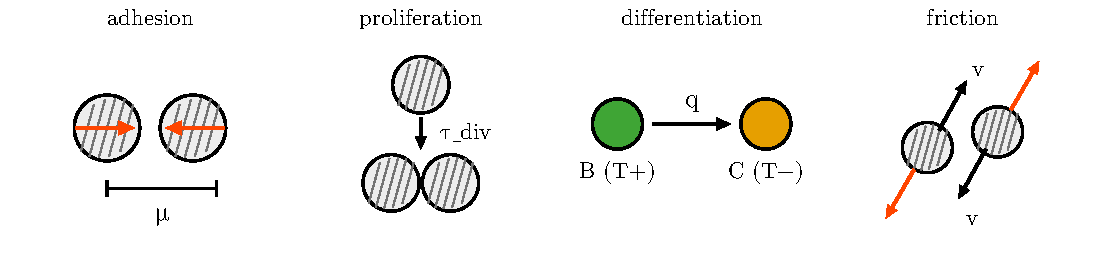
\includegraphics[width=\linewidth]{overview-A.pdf}
    \vspace{0.5em}
    \small
    \begin{itemize}
        \item Each cell is a sphere. Neighbours \textbf{attract and repel} each other, with strengths that depend on the state of both cells.
        \item Cells \textbf{divide} after a random time ($\B$ every 20\,h, $\C$ every 50\,h).
        \item $\B$ (T/Bra$^+$) cells \textbf{differentiate} into $\C$ (T/Bra$^-$) at a constant rate $q$.
        \item Two rigid \textbf{plates}, with some in-plane \textbf{friction} on the cells that touch them.
    \end{itemize}
\end{frame}


\begin{frame}{Mechanics}
    \begin{block}{Overdamped dynamics}
        \small
        \begin{equation*}
            \dot{\bx}_i = \bv_i \,, \qquad
            \bv_i = \frac{1}{\lambda n_i}\Big( \sum_j \mathbf{F}_{ij} + \alpha \sum_j \bv_j \Big)
        \end{equation*}
        \begin{equation*}
            \mathbf{F}_{ij} = f(d_{ij})\,\hat{\mathbf{r}}_{ij} \times
            \begin{cases}
                F_\text{rep}^{(s_i,s_j)} & d_{ij} \le 2r \\
                F_\text{att}^{(s_i,s_j)} & 2r < d_{ij} < 2\mu_{s_i s_j} r
            \end{cases}
            \qquad
            f(d) = \Big(\frac{2r}{d}-1\Big)\Big(\frac{2\mu r}{d}-1\Big)
        \end{equation*}
    \end{block}
    \pause
    \begin{block}{Plates}
        \small
        Rigid plates at $z=0$ and $z=L$, with $L = 2.1\,r\times(\text{number of layers})$. Cells touching a plate feel an extra in-plane drag $\lambda_\text{wall}$.
    \end{block}
    \pause
    \begin{block}{Simplifications}
        \small
        No $A$ state: at squeezing only $\B$ and $\C$ cells remain. No noise: cells move only because neighbours divide and push, and because adhesion changes with differentiation.
    \end{block}
\end{frame}


\begin{frame}{Initial condition and readout}
    \begin{columns}[c]
    \column{0.5\textwidth}
        \centering
        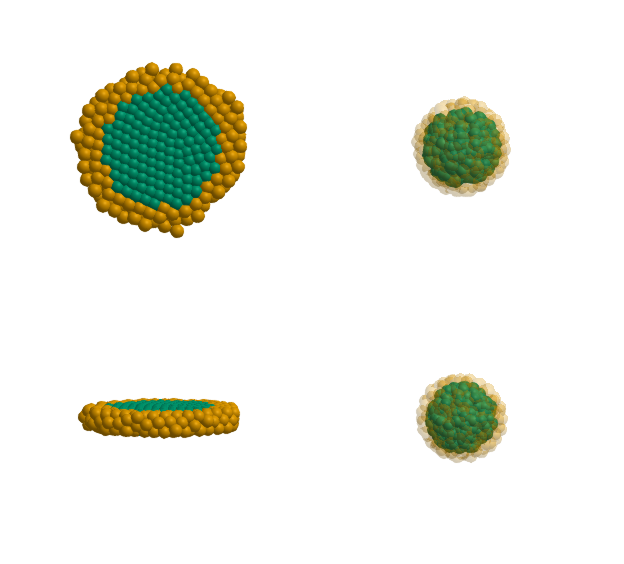
\includegraphics[width=\linewidth]{fig1_initial_condition.png}
    \column{0.48\textwidth}
        \small
        \begin{itemize}
            \item An already squeezed aggregate: grown between the plates and relaxed.
            \item A central core of $\B$ cells with $60\%$ of the cells; the rest are $\C$.
            \item The outcome is read when $20\%$ of the cells are $\B$, about $18$\,h later.
            \\ In the experiments T/Bra$^+$ falls from $60\%$ to $20\%$ between 72 and 96\,h.
        \end{itemize}
    \end{columns}
    \vspace{0.5em}
    {\scriptsize Left: 2 layers, top view cut at the mid-plane. Right: unconfined, $\C$ translucent. Both $N_0 = 600$.}
\end{frame}


\begin{frame}{Sanity checks}
    \begin{block}{Fusion}
        \small
        $\B\B$ and $\C\C$ doublets fuse into one sphere; $\B\C$ doublets glue but do not round up.
        \begin{center}
            \begin{tabular}{cc}
                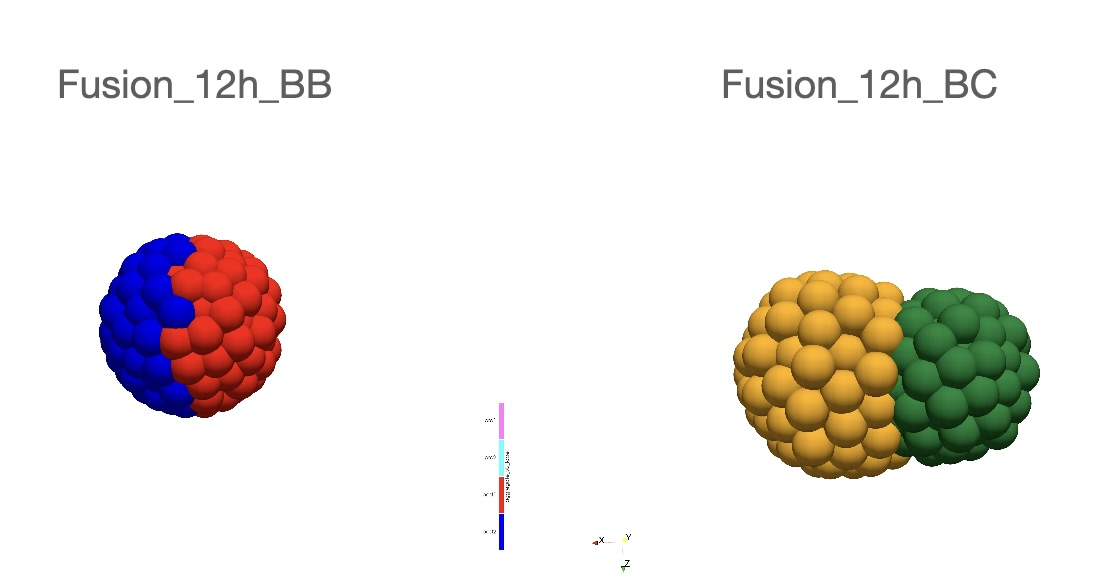
\includegraphics[height=4.5em]{fusions-relevant.jpeg} &
                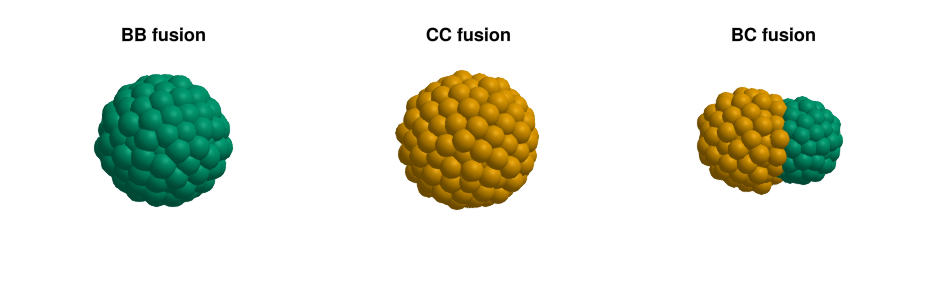
\includegraphics[height=4.5em]{fig5_fusion.png} \\
                {\scriptsize Expected} & {\scriptsize Model, after 24\,h}
            \end{tabular}
        \end{center}
    \end{block}
    \pause
    \begin{block}{Polarisation}
        \small
        Unconfined aggregates of up to $N_0 = 600$ cells polarise before $\B$ runs out.
        \begin{center}
            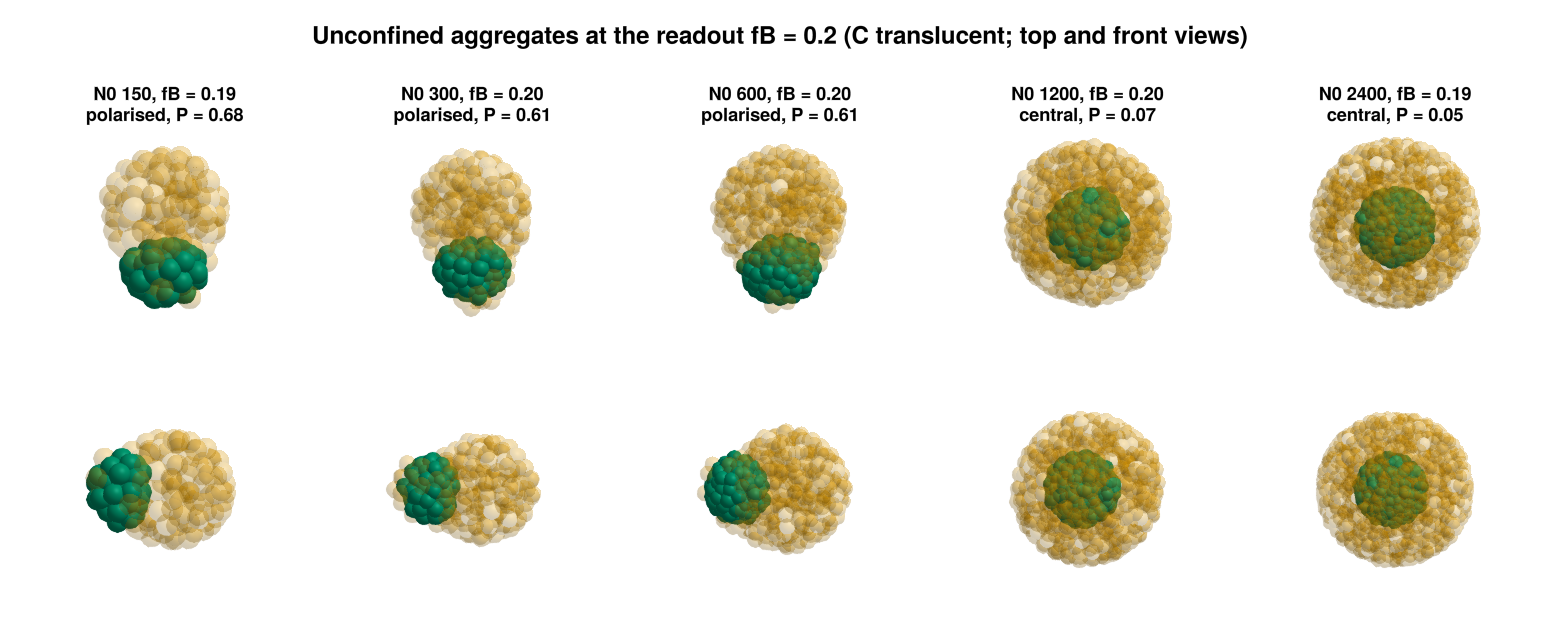
\includegraphics[width=0.7\linewidth]{fig4_unconfined.png}
        \end{center}
    \end{block}
\end{frame}



\section{Results}

\begin{frame}{The three behaviours}
    \centering
    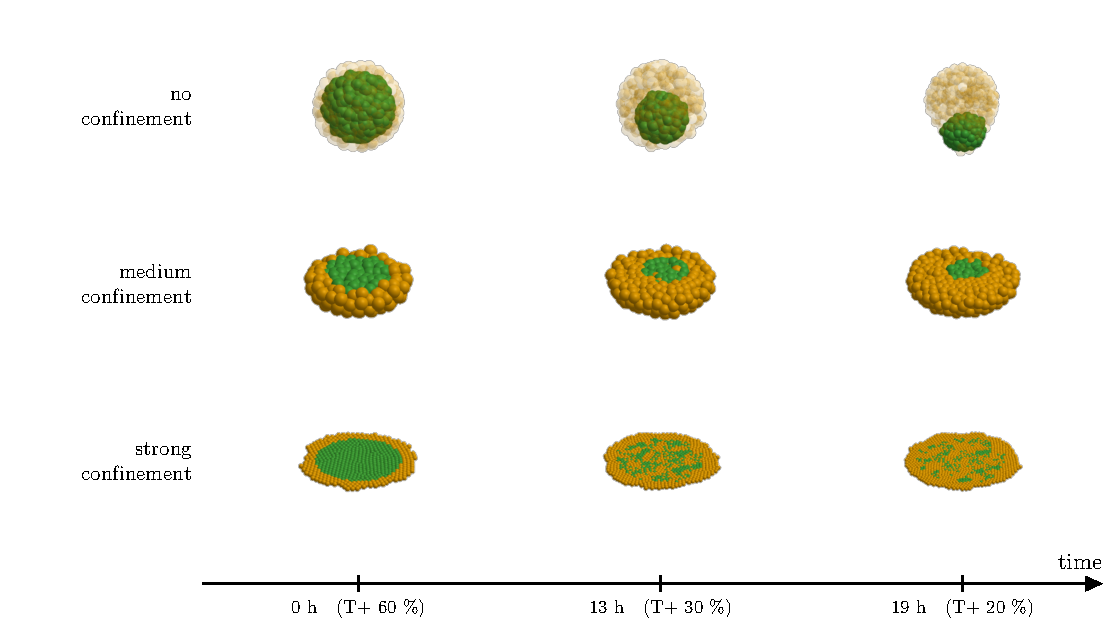
\includegraphics[width=\linewidth]{overview-B.pdf}
    \vspace{0.25em}
    {\small The same aggregate ($N_0 = 600$) with no, medium (4 layers) and strong (1 layer) confinement.}
\end{frame}


\begin{frame}{Patterns}
    \centering
    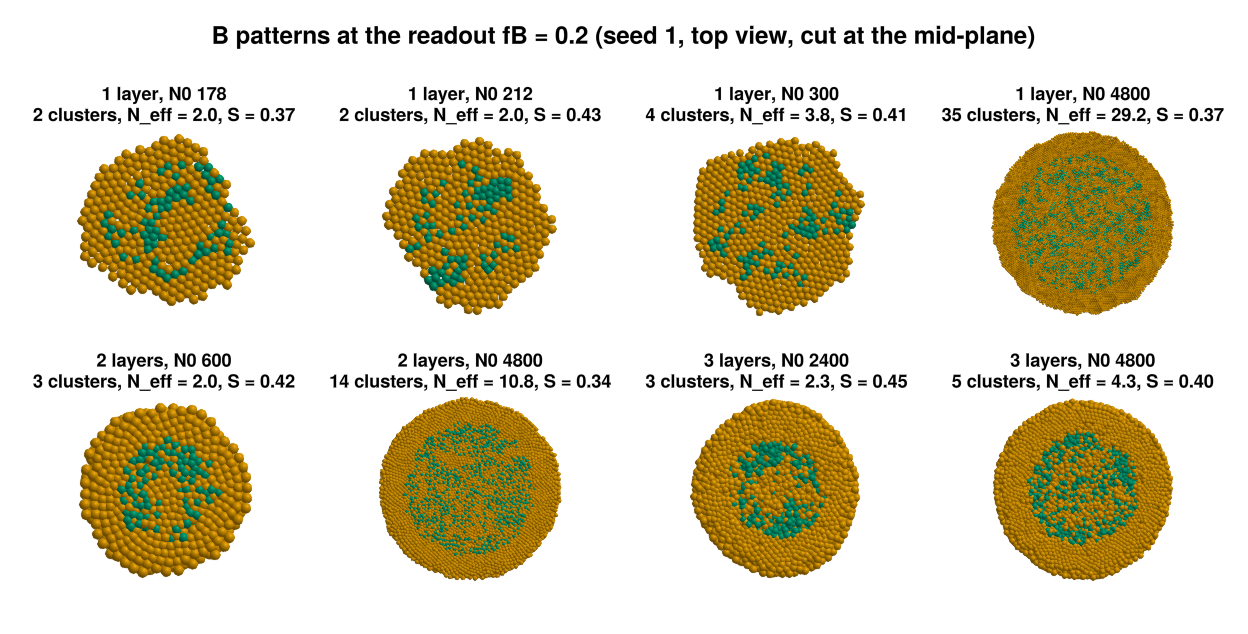
\includegraphics[width=0.62\linewidth]{fig3_patterns.png}
    \\ {\scriptsize From one to three layers, when $20\%$ of the cells are $\B$. Top view cut at the mid-plane.}
    \pause
    \vspace{0.5em}
    \begin{block}{}
        \small
        In thick slabs the core first hollows into a \textbf{ring}, which then breaks into islands.
        \begin{center}
            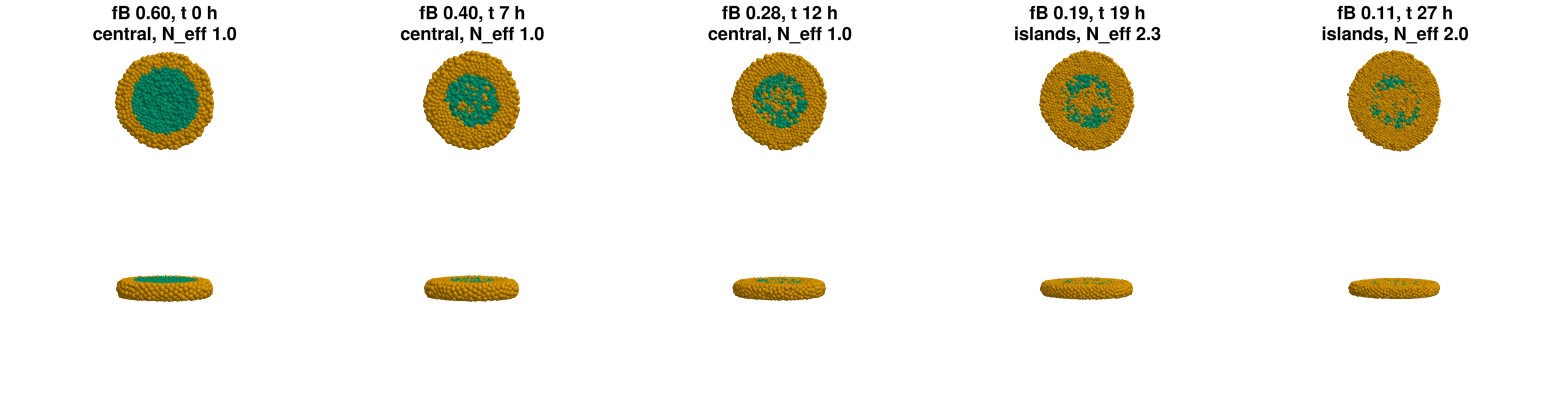
\includegraphics[width=0.9\linewidth]{ring-3layers.png}
        \end{center}
    \end{block}
\end{frame}


\begin{frame}{What makes thick slabs pattern}
    \small
    \begin{itemize}
        \item In one or two layers, new $\C$ cells inside the $\B$ core cannot get out and \textbf{split the core}.
        \item From three layers on, cells pass over and under each other: a cohesive core \textbf{squeezes the $\C$ cells out} and stays as one cluster.
    \end{itemize}
    \pause
    \begin{block}{The $\B$--$\B$ adhesion energy}
        \begin{itemize}
            \item Shortening the $\B$--$\B$ attraction range, $\mu_{BB}: 2 \to 1.9$, lowers $W_{BB}$ from $1.02$ to $0.79$, still above $W_{CC} = 0.65$. Large cores in thick slabs now open into rings.
            \item With $\mu_{BB} = 1.85$, $W_{BB} \approx W_{CC}$: $\B$ is no longer more cohesive than $\C$ and \textbf{dissolves} into it.
        \end{itemize}
    \end{block}
    \pause
    \centering
    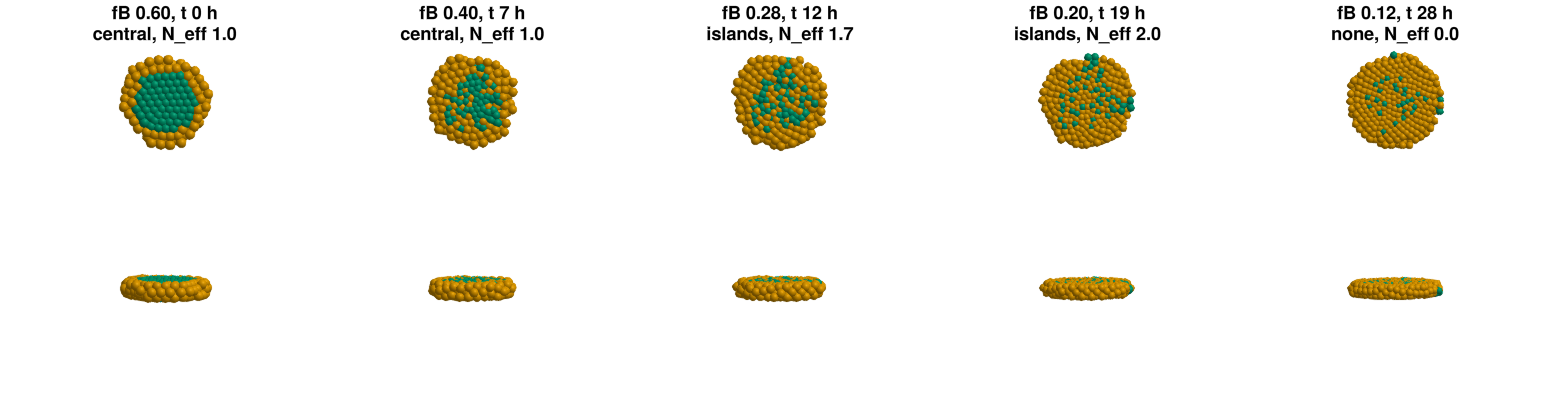
\includegraphics[width=0.75\linewidth]{dissolves-muBB1.8.png}
\end{frame}


\begin{frame}{Reading the outcome as in the experiments}
    \small
    From the positions and states when $20\%$ of the cells are $\B$:
    \begin{itemize}
        \item \textbf{Clusters}: the experiments' density-based clustering of $\B$ cells (radius $13\,\mu$m), and the effective number of clusters $N_\text{eff} = 1/\sum_k p_k^2$.
        \item \textbf{Polarisation}: $P = |\bar\bx_B - \bar\bx|/R$, with $R$ half the length along the longest axis.
    \end{itemize}
    \pause
    \begin{block}{Outcome}
        \begin{enumerate}
            \item \textbf{Polarised} if $P \ge 0.3$;
            \item \textbf{Clusters} if $N_\text{eff} \ge 1.5$;
            \item \textbf{Central cluster} otherwise (an unbroken ring counts as central).
        \end{enumerate}
    \end{block}
    \pause
    \begin{alertblock}{Changes for our smaller aggregates (10 to 100 times fewer cells)}
        Clusters of at least $10$ cells instead of $20$, and a core cell needs $50\%$ of $\B$ neighbours instead of $40\%$.
    \end{alertblock}
\end{frame}


\begin{frame}{Phase space}
    \centering
    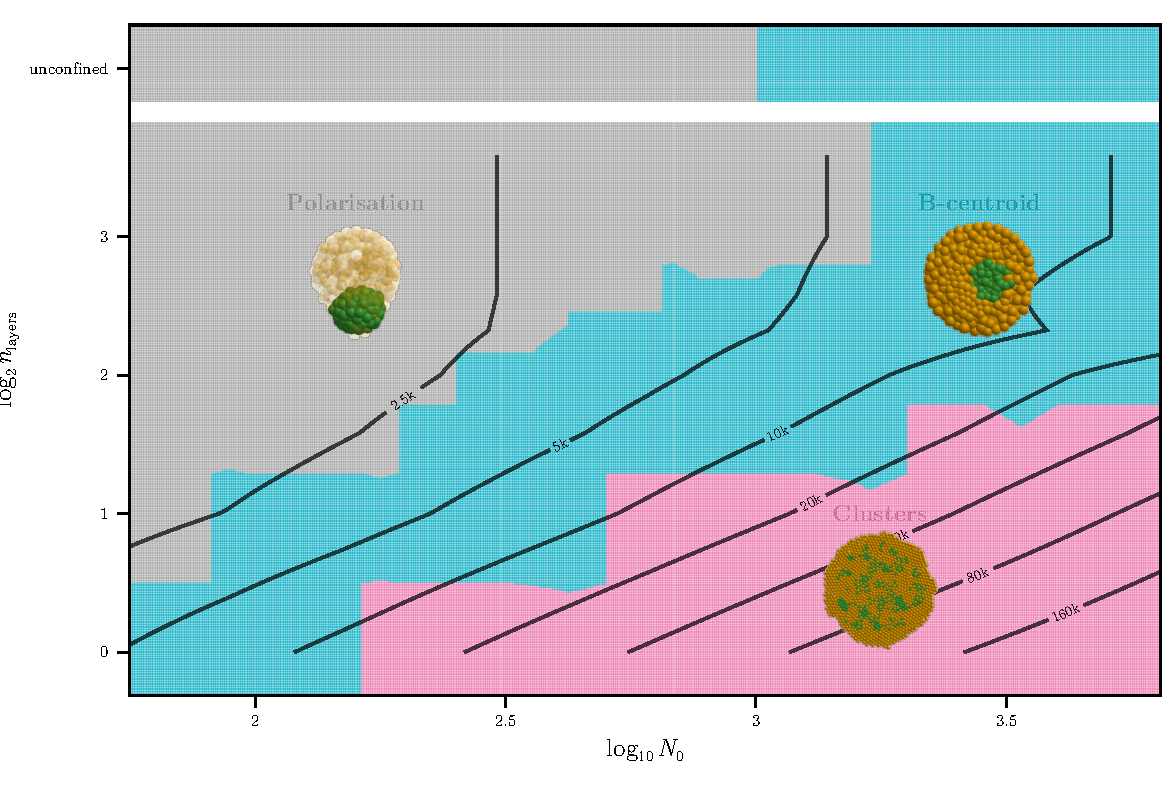
\includegraphics[height=0.72\textheight]{overview-C.pdf}
    \\ {\scriptsize Number of cells at squeezing against the number of layers, 2 or 3 simulations per point. Lines: area of the pancake at squeezing ($\mu$m$^2$).}
\end{frame}


\begin{frame}{The width of the pancake sets the threshold}
    \begin{columns}[c]
    \column{0.6\textwidth}
        \centering
        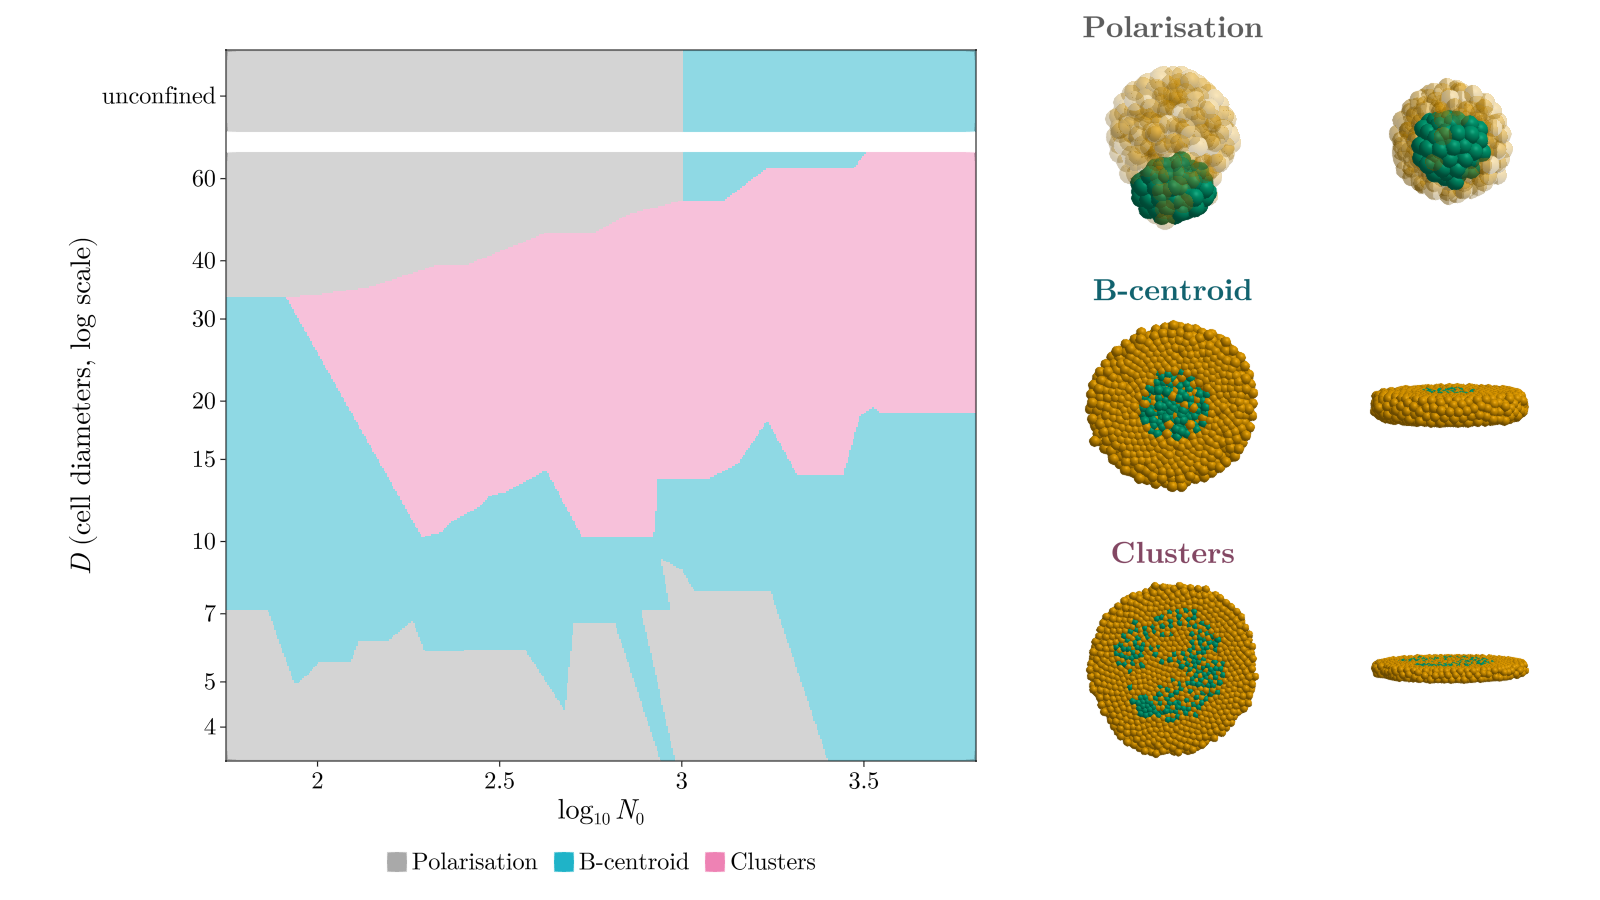
\includegraphics[width=\linewidth]{phase_space_diameter.png}
    \column{0.38\textwidth}
        \small
        \begin{itemize}
            \item The threshold in $N_0$ grows fast with thickness: from $\approx 160$ cells at one layer to $\approx 4000$ at four.
            \item<2-> Against the \textbf{diameter} of the pancake it barely moves: patterns appear at $8$ to $17$ cell diameters, roughly $80$ to $170\,\mu$m.
            \item<3-> A thicker slab simply needs more cells to reach the same width.
        \end{itemize}
    \end{columns}
\end{frame}


\begin{frame}{Differentiation is faster than mixing}
    \small
    The Damköhler number compares differentiation with cell mixing over a length $\ell$,
    \begin{equation*}
        \mathrm{Da} = \frac{q\,\ell^2}{D}.
    \end{equation*}
    \pause
    \begin{itemize}
        \item Measured in growing monolayers: $D \approx 1.5\,\mu\text{m}^2/\text{h}$ for $\B$ and $\C$ alike.
        \item A cell needs about $17$\,h to move one diameter, longer than a $\B$ cell lives ($\approx 14$\,h).
        \item<3-> Over the pancake, $\mathrm{Da} \approx 0.015\,A/\mu\text{m}^2$: the iso-area lines of the phase space are lines of constant $\mathrm{Da}$, and the pattern threshold sits at $\mathrm{Da}\approx 200$.
    \end{itemize}
    \pause
    \pause
    \begin{alertblock}{}
        The $\B$ pattern is set where the cells already are.
    \end{alertblock}
\end{frame}



\section{Conclusions}

\begin{frame}{Conclusions and open points}
    \small
    \begin{block}{Conclusions}
        \begin{itemize}
            \item One parameter set gives polarisation, a central cluster, rings and islands, and the right fusion behaviour.
            \item The cohesion of the $\B$ tissue decides whether thick slabs pattern.
            \item The pattern threshold is set by the width of the pancake, not by its thickness.
        \end{itemize}
    \end{block}
    \pause
    \begin{alertblock}{Open points}
        \begin{itemize}
            \item Large unconfined aggregates neither pattern nor polarise before $\B$ runs out.
            \item $\mu_{BB} = 1.9$ is close to the point where $\B$ dissolves ($1.85$).
            \item Are the diameter at squeezing and the cell diffusion coefficient measured in the experiments? They would test the threshold and $\mathrm{Da}$ directly.
        \end{itemize}
    \end{alertblock}
\end{frame}


\section{}
\begin{frame}
    \centering
    \vfill
    \huge
    Thank you for your attention!
    \\[0.25em] Gràcies per la vostra atenció!
    \vfill
\end{frame}



\appendix
\setbeamertemplate{page number in head/foot}{}   % no slide numbers in the appendix

\begin{frame}{Phase space read later}
    \centering
    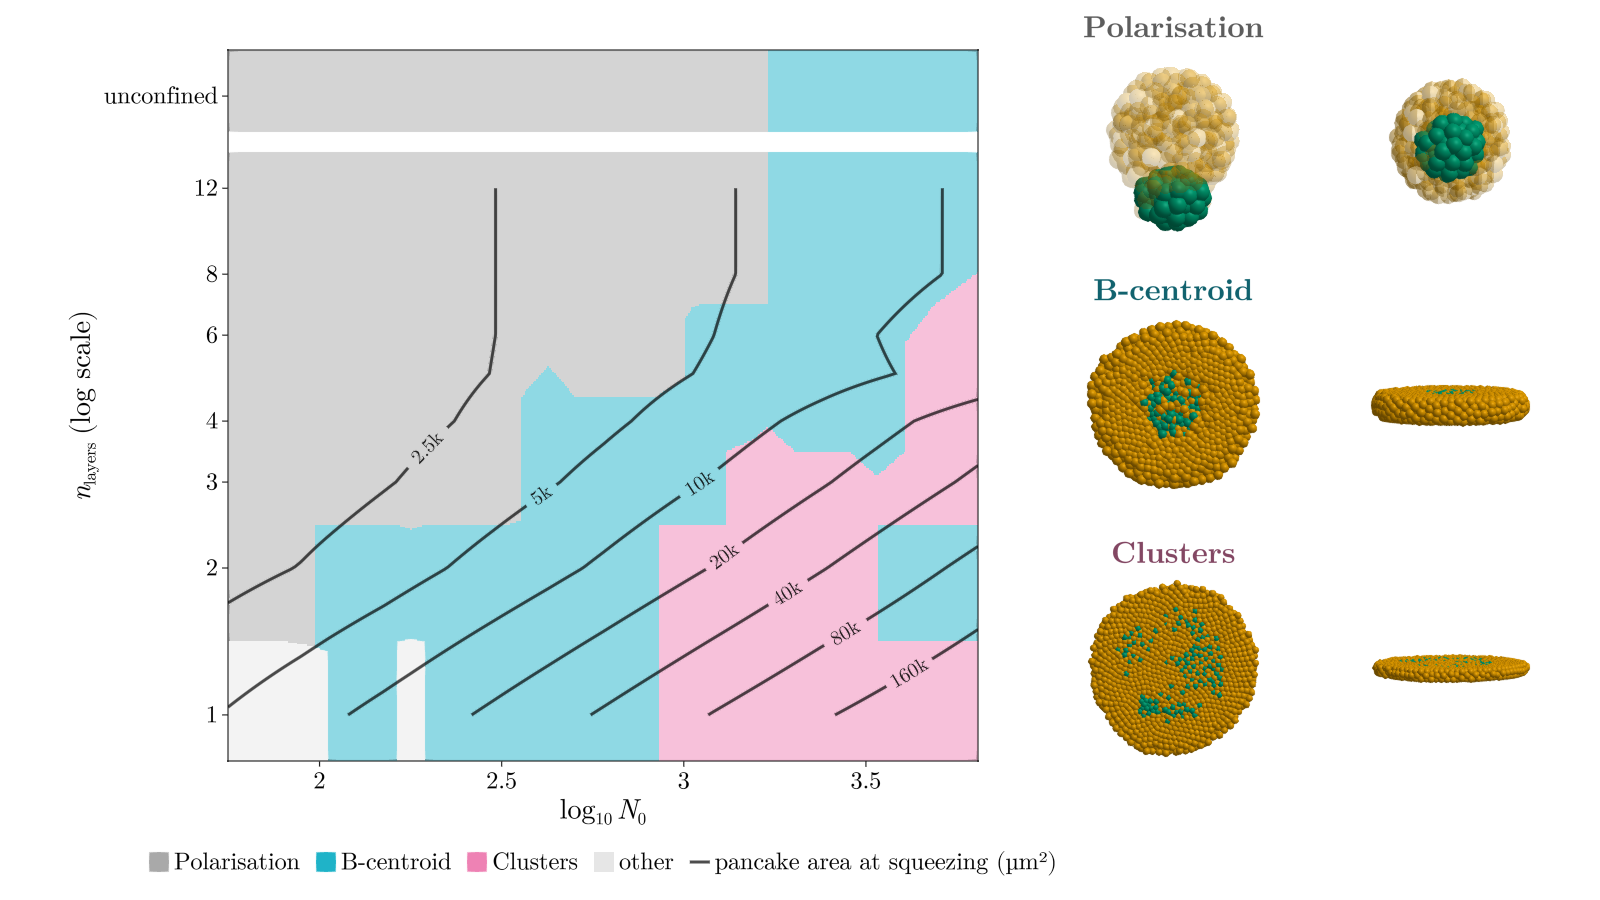
\includegraphics[width=0.9\linewidth]{phase_space_late.png}
    \\ {\small The same simulations when $12\%$ of the cells are $\B$: rings break into islands, larger aggregates polarise late, and the smallest monolayer patterns shrink back to a central cluster.}
\end{frame}


\begin{frame}{Mean squared displacement}
    \centering
    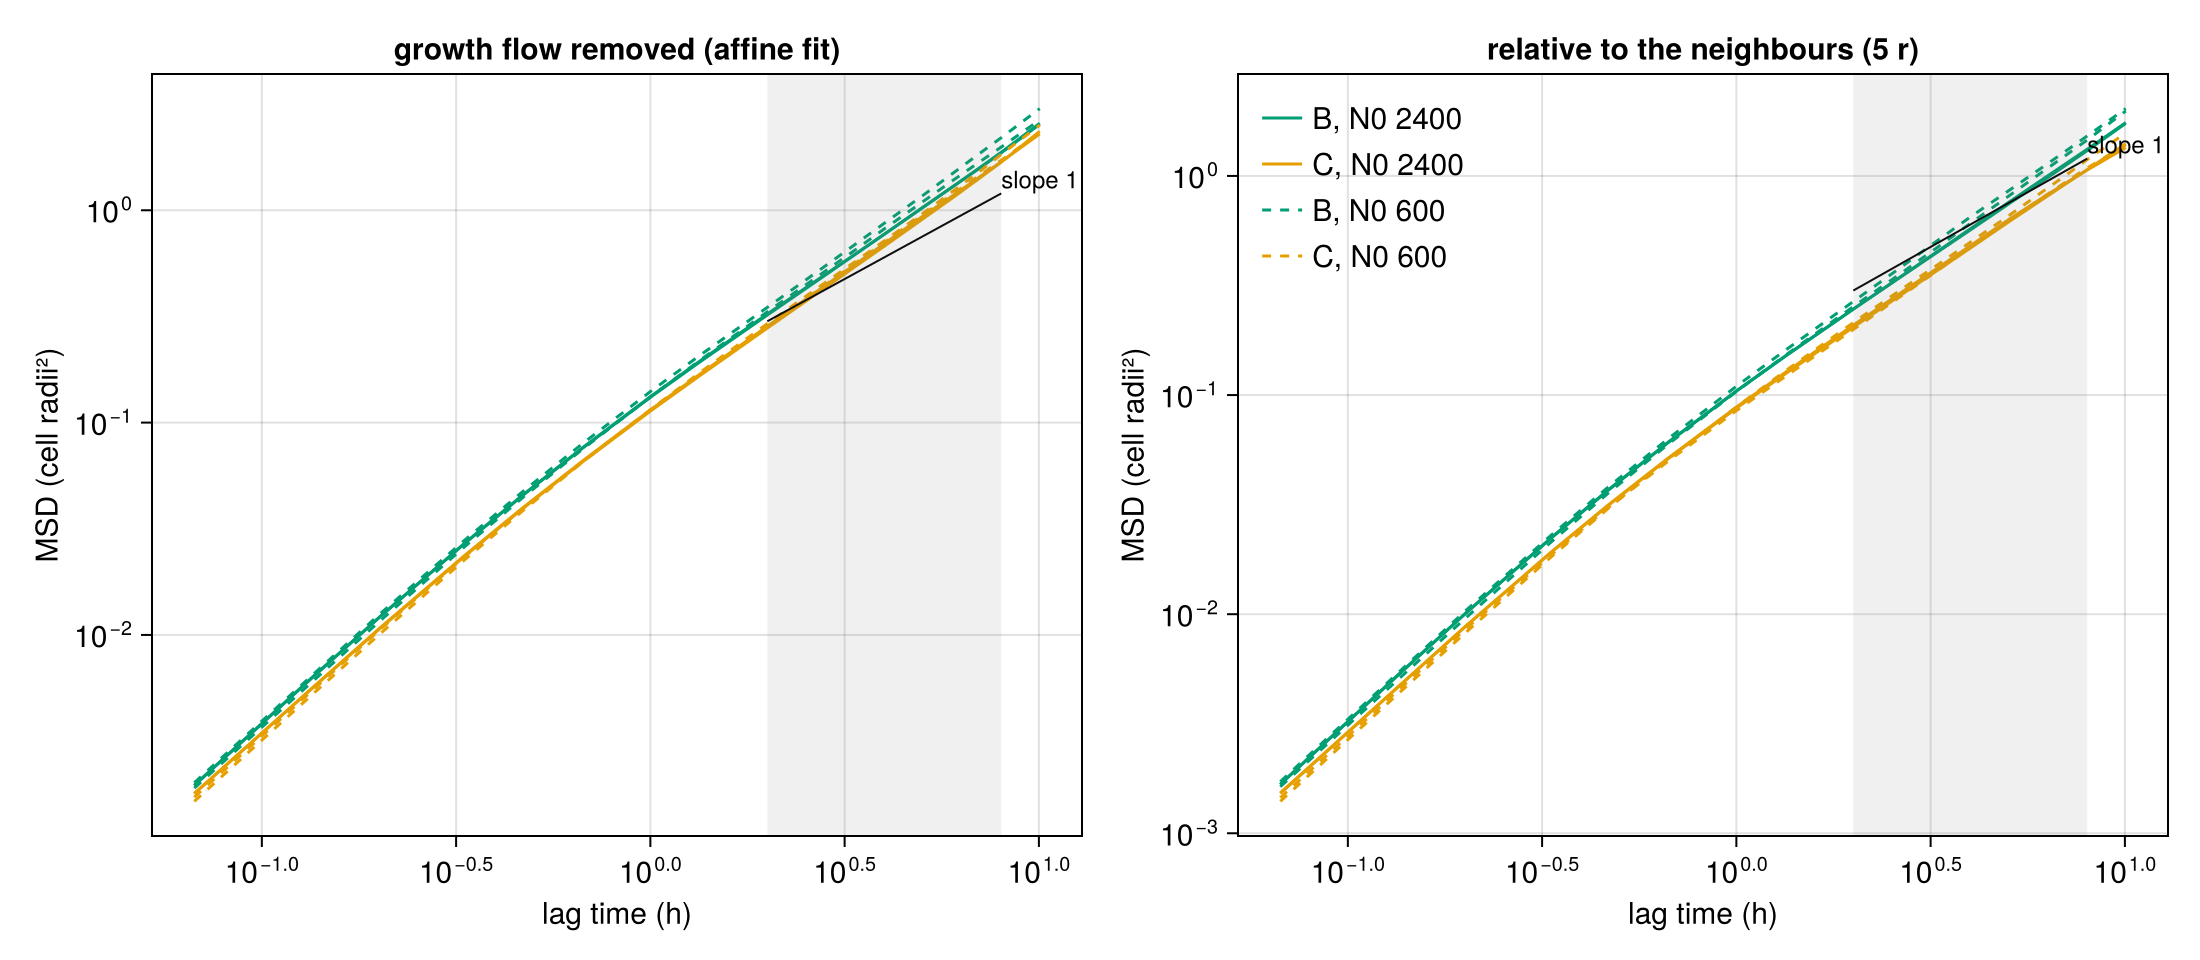
\includegraphics[width=\linewidth]{msd.png}
    \\ {\small $\B$ (green) and $\C$ (yellow) cells in growing monolayers ($N_0 = 600$ dashed, $2400$ solid). Left: growth flow removed with an affine fit; right: relative to the neighbours within $5r$. Shaded: the fitted lag times.}
\end{frame}


\begin{frame}{Parameters}
    \small
    \centering
    \begin{tabular}{lll}
        \hline
        \textbf{Symbol} & \textbf{Description} & \textbf{Value} \\
        \hline
        $r$ & Radius & $1 = 5\,\mu$m \\
        $\lambda$, $\alpha$ & Friction, cell-cell friction & $1$, $0.9$ \\
        $\tau_\text{div}^B$, $\tau_\text{div}^C$ & Division times & $300$, $750$ ($20$\,h, $50$\,h) \\
        $q$ & $\B\to\C$ rate & $0.004667$ \\
        $\mu_{BB}$, $\mu_{BC}$, $\mu_{CC}$ & Force range factors & $1.9$, $2$, $2.14$ \\
        $F_\text{rep}^{BB}$, $F_\text{rep}^{BC}$, $F_\text{rep}^{CC}$ & Repulsion & $4.5$, $3$, $6$ \\
        $F_\text{att}^{BB}$, $F_\text{att}^{BC}$, $F_\text{att}^{CC}$ & Attraction & $6.4$, $1.6$, $3$ \\
        $\lambda_\text{wall}$ & Plate friction & $1.5$ \\
        $L$ & Plate gap & $2.1\,r\times$ layers \\
        $T_0$ & Time unit & $4$\,min \\
        \hline
    \end{tabular}
\end{frame}

\end{document}
